    \subsection{DONE}
\subsection{DONE}
\subsection{DONE}
\subsection{DONE}
\subsection{}
\subsubsection{DONE}
We fixed the front wheel to remove the singularity of K. $q_{\text{init}}$  was given as:

\begin{equation}\label{eq:4.5.1}
    \begin{split}
        q_{\text{init}} = 
        \begin{pmatrix}
            &\theta_{\text{Frame}} = 0\\
            &x_{\text{Frame}} = 0\\
            &y_{\text{Frame}} = 0.22\\
            &\theta_{\text{Wheel Back}} = 0\\
            % &\theta_{\text{Wheel Front}} = 0\\
            &\theta_{\text{Tire Front}} = 0\\
            &\theta_{\text{Tire Back}} = 0\\
            &y_{\text{Tire Front}} = 0.21\\
            &y_{\text{Tire Back}} = 0.21\\
            &\beta_{\text{Link Back}} = \pi\\
            &\beta_{\text{Link Front}} = 0
        \end{pmatrix}
    \end{split}
\end{equation}

Which represents this position:

\begin{figure}[ht]
    \centering
    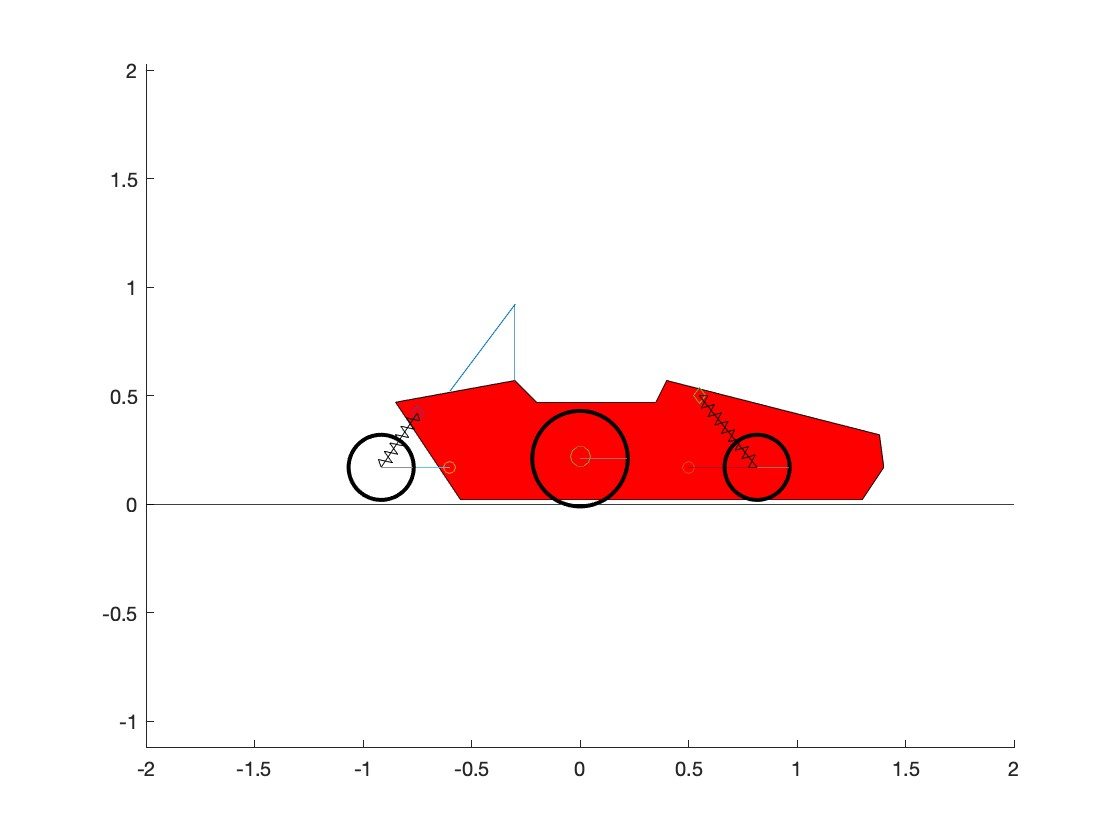
\includegraphics[scale=0.235]{images/q_init_1.jpg}
    \caption{Initial Position 1}
    %label always in the end
    \label{fig:init_1}
\end{figure}


This resulted in the equilibrium:

\begin{equation}\label{eq:4.5.2}
    \begin{split}
        q_{\text{equilibrium 1}} = 
        \begin{pmatrix}
            &\theta_{\text{Frame}} = -1.3896e-02 = -0.014\\
            &x_{\text{Frame}} =  -8.1104e-01 = -0.811\\
            &y_{\text{Frame}} = 2.1926e-01 = -0.219\\
            &\theta_{\text{Wheel Back}} = 7.8437e+00 = 7.844\\
            % &\theta_{\text{Wheel Front}} = 0\\
            &\theta_{\text{Tire Front}} = 2.2254e-21 \approx 0\\
            &\theta_{\text{Tire Back}} = 7.8437e+00 = 7.844\\
            &y_{\text{Tire Front}} = 2.1883e-01 = 0.219\\
            &y_{\text{Tire Back}} = 2.1895e-01 = 0.219\\
            &\beta_{\text{Link Back}} = 3.0209e+00 = 3.021\\
            &\beta_{\text{Link Front}} = 1.6787e-01 = 0.168
        \end{pmatrix}
    \end{split}
\end{equation}
Which is visualized by this figure:

\begin{figure}[ht]
    \centering
    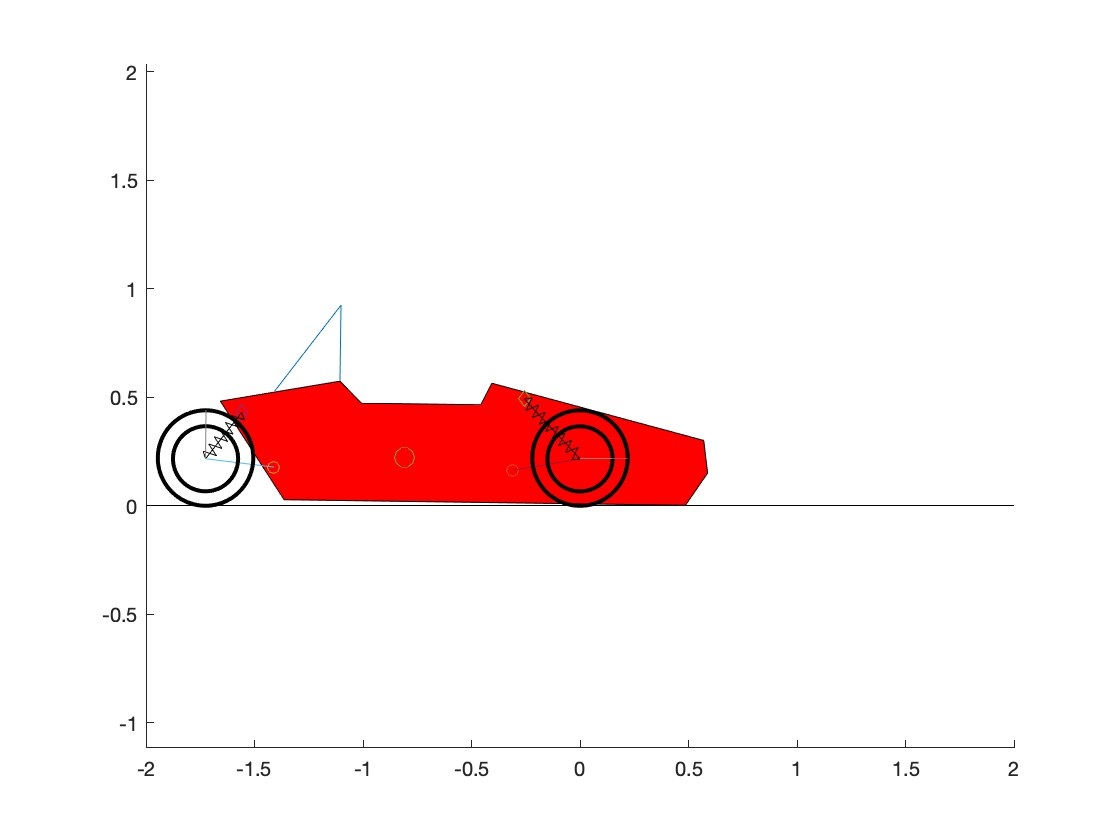
\includegraphics[scale=0.235]{images/Equilibrium1.jpg}
    \caption{Equilibrium Position 1}
    %label always in the end
    \label{fig:eq_1}
\end{figure}

\noindent In this example the choice of initial generalized coordinates was obviously very good. For the first task of this assignment the goal is to find two more (probably bad) equilibria.

The eigenvalues of the stiffness matrix are:




\subsubsection{Different Equilibrium states}

The first alternative is luckily already given in the code. Again we fix the front wheel's rotation and start with the initial state:

\begin{equation}\label{eq:4.5.3}
    \begin{split}
        q_{\text{init}} = 
        \begin{pmatrix}
            &\theta_{\text{Frame}} = \pi/2\\
            &x_{\text{Frame}} = 0\\
            &y_{\text{Frame}} = 90\\
            &\theta_{\text{Wheel Back}} = 0\\
            % &\theta_{\text{Wheel Front}} = 0\\
            &\theta_{\text{Tire Front}} = 0\\
            &\theta_{\text{Tire Back}} = 0\\
            &y_{\text{Tire Front}} = 1.90\\
            &y_{\text{Tire Back}} = 0.21\\
            &\beta_{\text{Link Back}} = -\pi/2\\
            &\beta_{\text{Link Front}} = \pi/2
        \end{pmatrix}
    \end{split}
\end{equation}

Which represents this position:


\begin{figure}[ht]
    \centering
    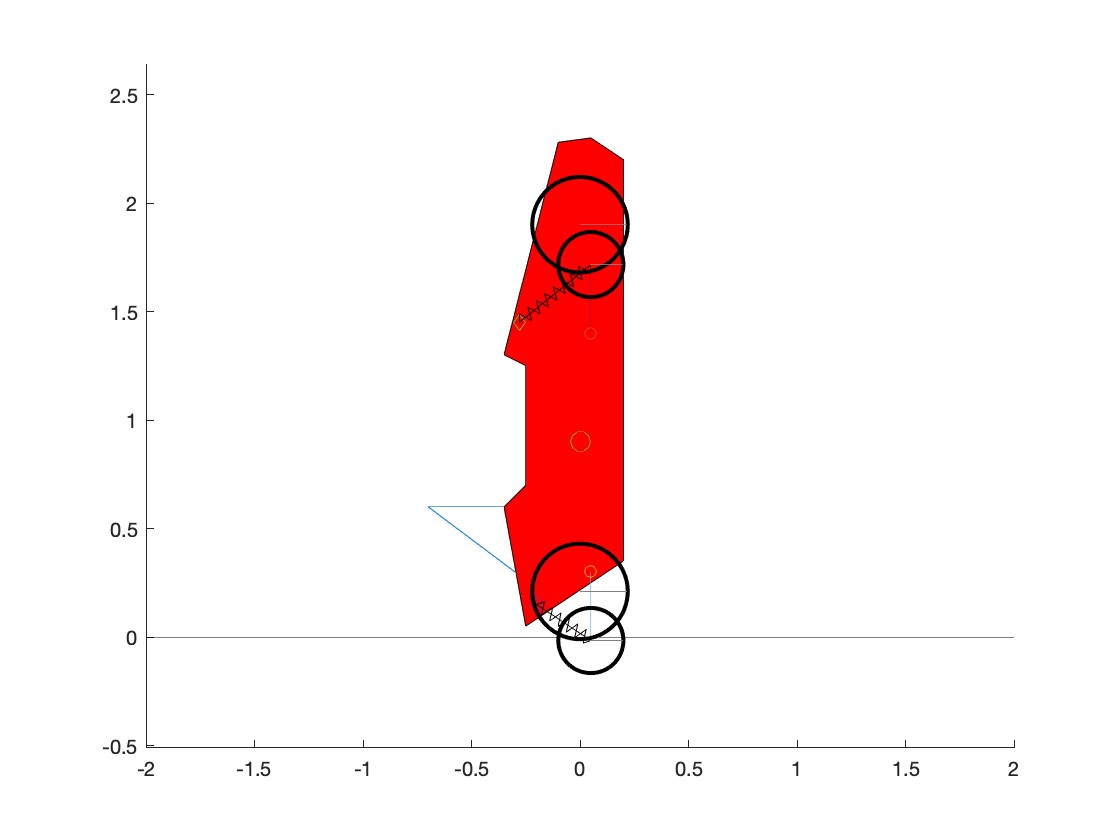
\includegraphics[scale=0.235]{images/q_init_2.jpg}
    \caption{Initial Position 2}
    %label always in the end
    \label{fig:init_2}
\end{figure}
\noindent Note: in the code provided $\theta_{\text{Frame}}$ was $\pi$ which was a different initial set of gen. coord. but converged to the same solution\\
\vspace{2mm}

\noindent As can be seen, this is obviously not a good choice of initial coordinates.

This setting converges to:

\begin{equation}\label{eq:4.5.4}
    \begin{split}
        q_{\text{init}} = 
        \begin{pmatrix}
            &\theta_{\text{Frame}} = 1.5248e+00\\
            &x_{\text{Frame}} = -6.9703e-02\\
            &y_{\text{Frame}} = 1.1280e+00\\
            &\theta_{\text{Wheel Back}} = 3.0427e-01\\
            % &\theta_{\text{Wheel Front}} = 0\\
            &\theta_{\text{Tire Front}} = 2.9622e-24\\
            &\theta_{\text{Tire Back}} = 3.0427e-01\\
            &y_{\text{Tire Front}} = 1.9414e+00\\
            &y_{\text{Tire Back}} = 2.1777e-01\\
            &\beta_{\text{Link Back}} = -1.6327e+00\\
            &\beta_{\text{Link Front}} = 1.5811e+00
        \end{pmatrix}
    \end{split}
\end{equation}

Which looks as follows:

\begin{figure}[ht]
    \centering
    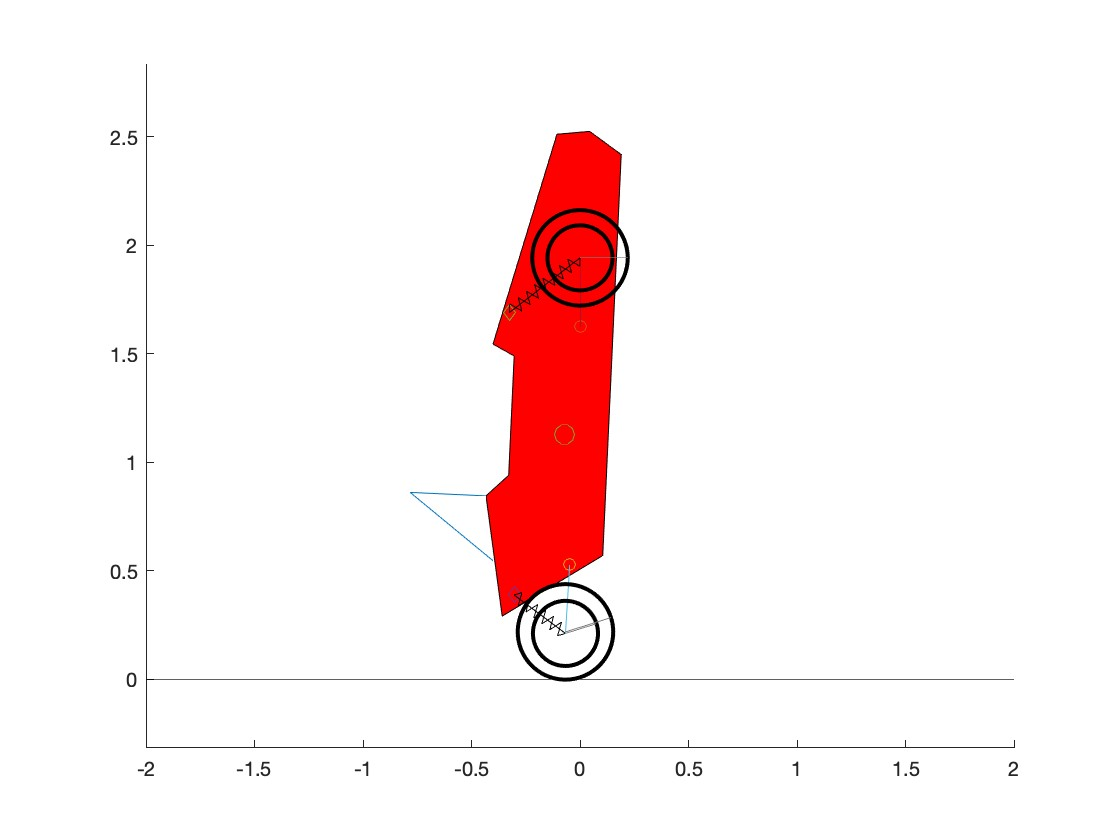
\includegraphics[scale=0.235]{images/Equilibrium2.jpg}
    \caption{Equilibrium Position 2}
    %label always in the end
    \label{fig:eq_2}
\end{figure}

The code example which has even worse initial conditions:

\begin{equation}\label{eq:4.5.5}
    \begin{split}
        q_{\text{init}} = 
        \begin{pmatrix}
            &\theta_{\text{Frame}} = \pi\\
            &x_{\text{Frame}} = 0\\
            &y_{\text{Frame}} = 90\\
            &\theta_{\text{Wheel Back}} = 0\\
            % &\theta_{\text{Wheel Front}} = 0\\
            &\theta_{\text{Tire Front}} = 0\\
            &\theta_{\text{Tire Back}} = 0\\
            &y_{\text{Tire Front}} = 1.90\\
            &y_{\text{Tire Back}} = 0.21\\
            &\beta_{\text{Link Back}} = -\pi/2\\
            &\beta_{\text{Link Front}} = \pi/2
        \end{pmatrix}
    \end{split}
\end{equation}

And looks like this:

\begin{figure}[ht]
    \centering
    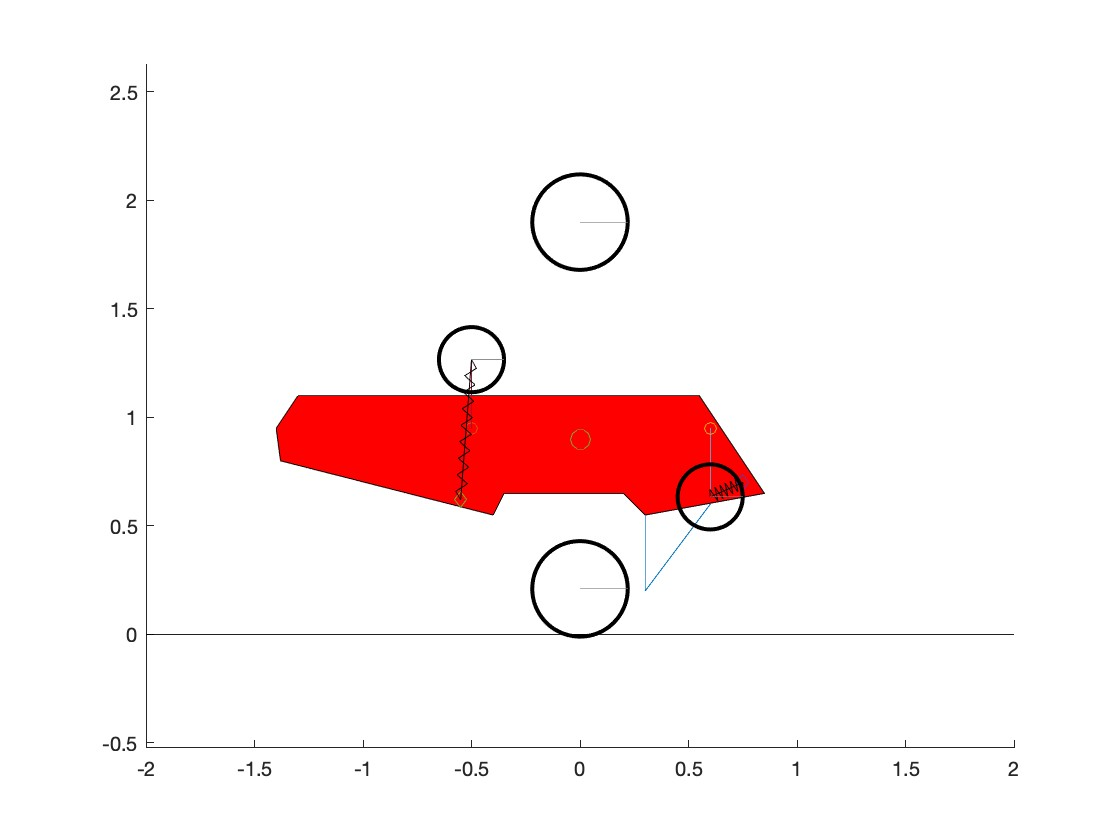
\includegraphics[scale=0.235]{images/q_init_3.jpg}
    \caption{Initial Position 3}
    %label always in the end
    \label{fig:init_3}
\end{figure}

Converges to:

\begin{equation}\label{eq:4.5.6}
    \begin{split}
        q_{\text{init}} = 
        \begin{pmatrix}
            &\theta_{\text{Frame}} = 2.0225e+00\\
            &x_{\text{Frame}} =  -1.2734e-01\\
            &y_{\text{Frame}} = 6.3440e-01\\
            &\theta_{\text{Wheel Back}} = 5.5591e-01\\
            % &\theta_{\text{Wheel Front}} = 0\\
            &\theta_{\text{Tire Front}} =  2.0275e-25\\
            &\theta_{\text{Tire Back}} = 5.5591e-01\\
            &y_{\text{Tire Front}} = 1.2043e+00\\
            &y_{\text{Tire Back}} = 2.1777e-01\\
            &\beta_{\text{Link Back}} = -3.4446e+00\\
            &\beta_{\text{Link Front}} = 3.1586e-01
        \end{pmatrix}
    \end{split}
\end{equation}
\clearpage%HERE
Which represents:

\begin{figure}[ht]
    \centering
    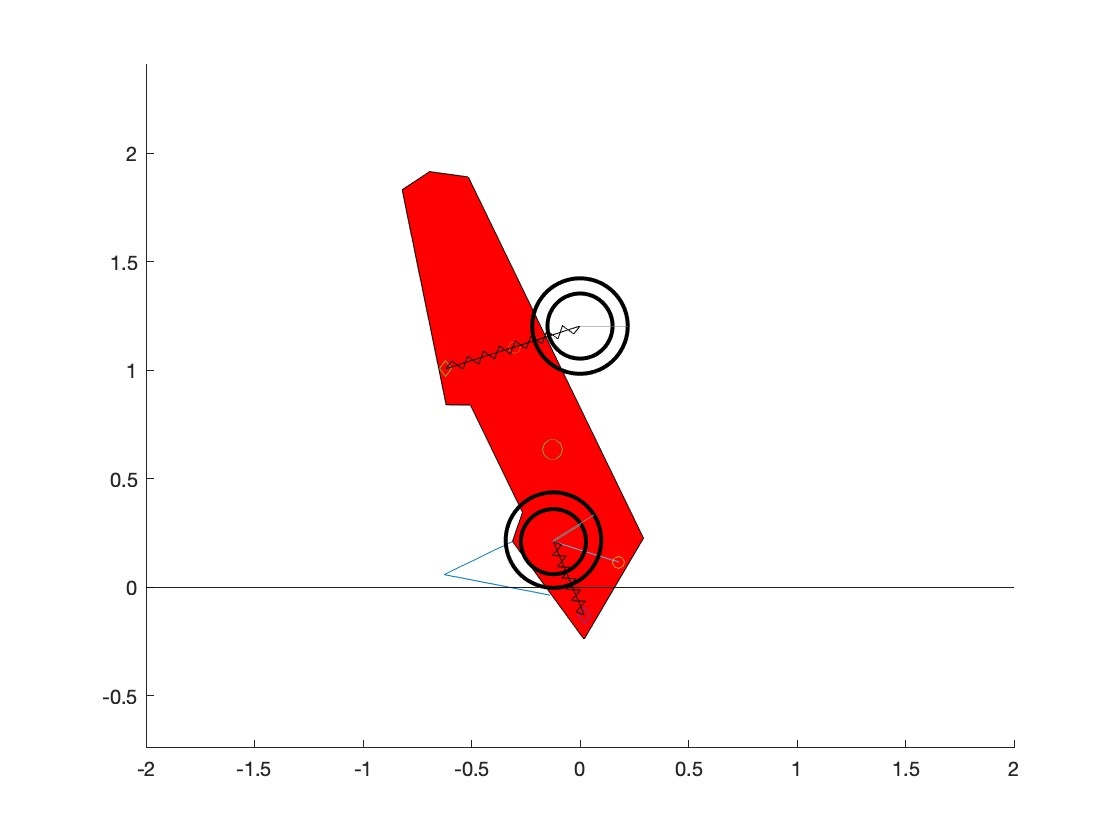
\includegraphics[scale=0.235]{images/Equilibrium3.jpg}
    \caption{Equilibrium Position 3}
    %label always in the end
    \label{fig:eq_3}
\end{figure}

\subsection{Analysis}
As we are not considering drag yet we have a conservative, scleronomic system. For an equilibrium in such a system to be stabel we need that $\text{K}_{\text{eq}}$ must be positive definite. Aka the eigenvalues of $\text{K}_{\text{eq}}$ must be real and positive.

Looking at the eigenvalues for the first case:
\begin{equation}\label{eq:normal_eigenfrequencies}
    \begin{split}
        \begin{pmatrix}
            1.6913e-07\\
            2.1774e+00\\
            2.2340e+00\\
            3.0009e+01\\
            3.0821e+01\\
            3.4894e+01\\
            3.5642e+01\\
            6.8555e+01\\
            6.8673e+01\\
            1.3035e+02\\
            1.3036e+02
        \end{pmatrix}
    \end{split}
\end{equation}

We can see that they are indeed all positive and real. Thus \ref{eq:4.5.2} is a stable equilibrium. This represents logical assumptions as the car staying in horizontal position is as we know a stable equilibrium.\vspace{3mm}\\

For the second equilibrium we get the following eigenvalues:

\begin{equation}
    \begin{pmatrix}
        0.0000e+00 + 4.9405e-01i\\
        0.0000e+00 + 1.2122e-07i\\
        4.4151e+00 + 0.0000e+00i\\
        7.1552e+00 + 0.0000e+00i\\
        7.4830e+00 + 0.0000e+00i\\
        4.3728e+01 + 0.0000e+00i\\
        4.3983e+01 + 0.0000e+00i\\
        6.3302e+01 + 0.0000e+00i\\
        7.2017e+01 + 0.0000e+00i\\
        7.2124e+01 + 0.0000e+00i\\
        1.2904e+02 + 0.0000e+00i
    \end{pmatrix}
\end{equation}

Where we can see that the eigenvalues ar of complex nature. Mainly the first one

Lastly for the third setting we have the following eigenvalues:

\begin{equation}
    \begin{pmatrix}
        0.0000e+00 + 4.9405e-01i\\
        1.9956e-07 + 0.0000e+00i\\
        4.4151e+00 + 0.0000e+00i\\
        7.1552e+00 + 0.0000e+00i\\
        7.4830e+00 + 0.0000e+00i\\
        4.3728e+01 + 0.0000e+00i\\
        4.3983e+01 + 0.0000e+00i\\
        6.3302e+01 + 0.0000e+00i\\
        7.2017e+01 + 0.0000e+00i\\
        7.2124e+01 + 0.0000e+00i\\
        1.2904e+02 + 0.0000e+00i
    \end{pmatrix}
\end{equation}

Where we see again, that we have complex eigenvalues denoting an unstable equilibrium.

% As we are working with a first order linearization of the dynamics of the system we have to stay in the proximity of the desired state of convergence. So a horizontal car with the initial conditions as seen in equation \ref{eq:4.5.1} will converge to a reasonable solution. \\\vspace{3mm}

% \noindent Initial conditions like a 90° or 180° rotation of the frame can converge to a local solution as seen in Figure \ref*{fig:eq_3}\\\vspace{3mm}

% \noindent The equilibrium from figure \ref{fig:eq_1} surely is stable as we all know it from reality. The two alternatives however are not stable. This can be seen from the example in fig \ref{fig:init_4} when the angle of the frame is between 0 and 90°:
\clearpage %HERE
Another interesting example is the one seen in fig \ref{fig:init_4}:



\begin{figure}[ht]
    \centering
    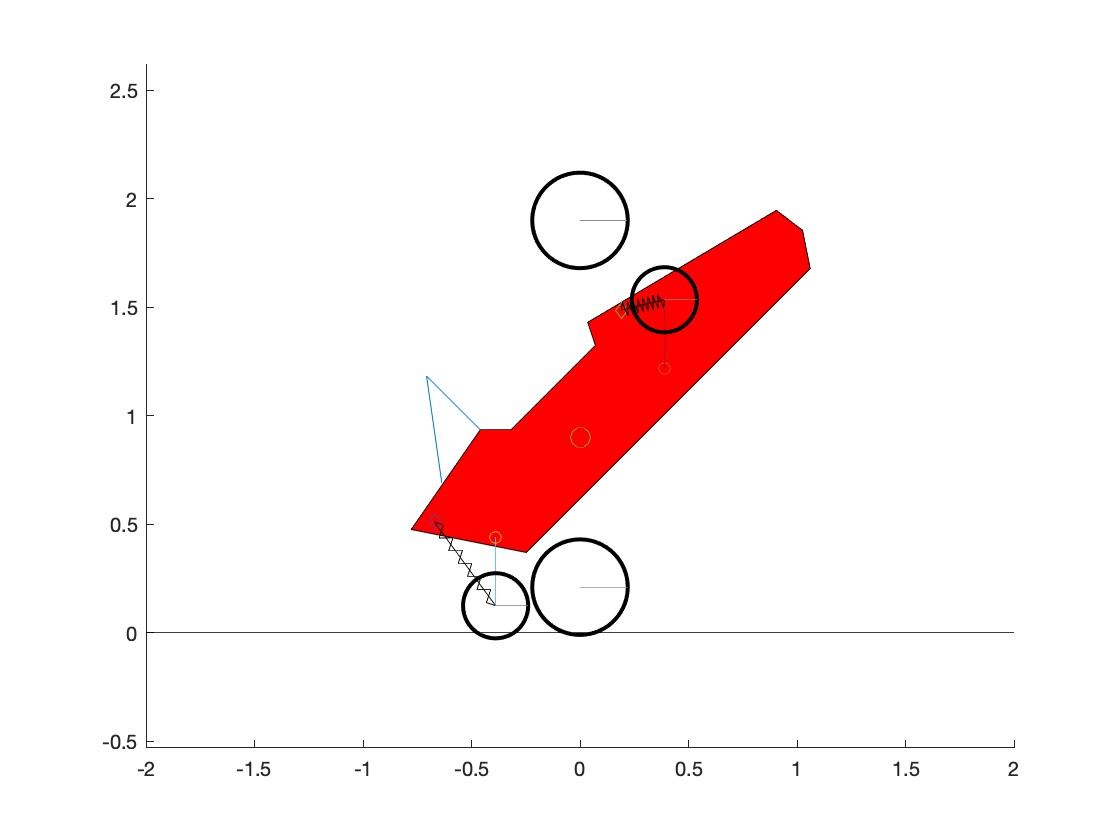
\includegraphics[scale=0.235]{images/q_init_4.jpg}
    \caption{Initial Position 4}
    %label always in the end
    \label{fig:init_4}
\end{figure}

When we start from the tilted starting position of \ref{fig:init_2} but changing merely the frame angle to a smaller $\pi/4$ we can see that it converges to something quite reasonable looking.
\begin{figure}[ht]
    \centering
    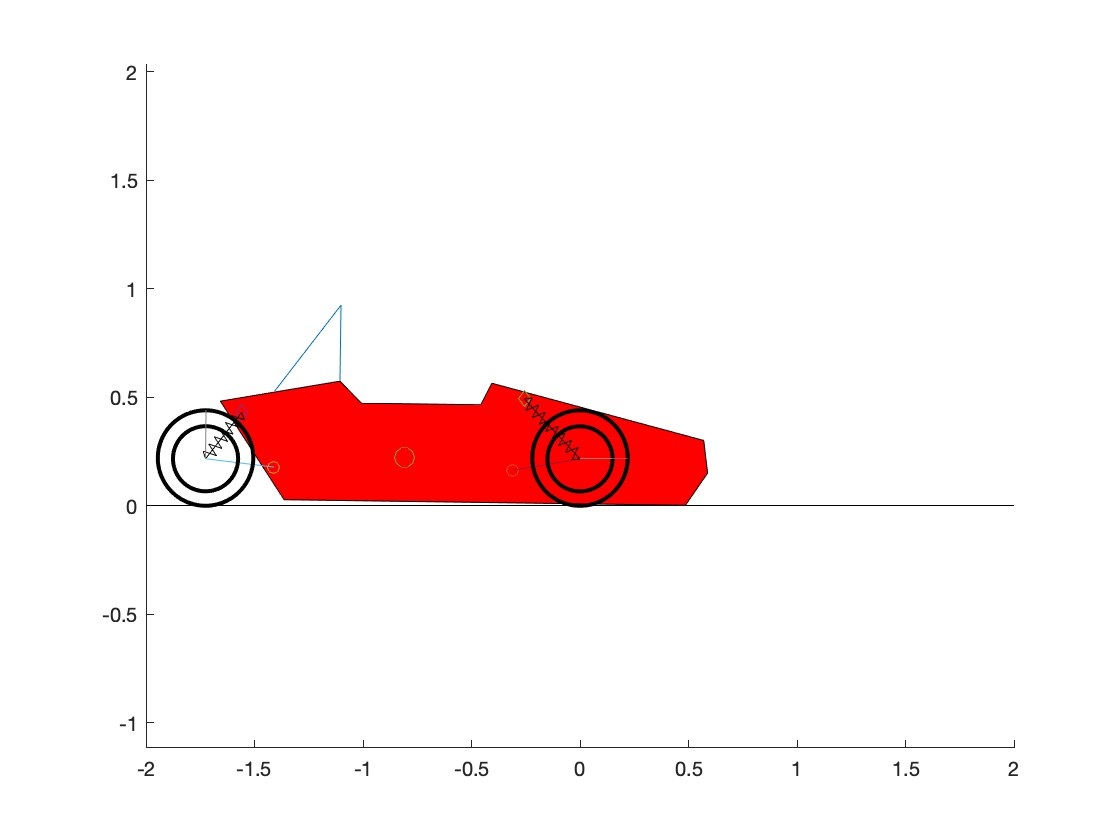
\includegraphics[scale=0.235]{images/Equilibrium4.jpg}
    \caption{Equilibrium Position 4}
    %label always in the end
    \label{fig:eq_4}
\end{figure}

And indeed when looking at the eigenvalues:

\begin{equation}
    \begin{pmatrix}
        2.5694e-07\\
        2.1774e+00\\
        2.2340e+00\\
        3.0009e+01\\
        3.0821e+01\\
        3.4894e+01\\
        3.5642e+01\\
        6.8555e+01\\
        6.8673e+01\\
        1.3035e+02\\
        1.3036e+02
    \end{pmatrix}
\end{equation}

We see that it's a stable equilibrium. From this we can take away that a perturbation from a stable equilibrium that is small enough will converge to the stable equilibrium.   
\subsection{Linearized Equations - DONE}
\subsection{Eigenmodes and Eigenfrequencies}

Looking at the eigenfrequencies in equation (\ref{eq:normal_eigenfrequencies}) we can see that the dominant ones with the large motion impact seem to be the first as well as the second and third.

The eigenmodes associated with these frequencies are:

\begin{equation}
    \begin{split}
        \begin{pmatrix}
            6.0858e-01\\
            9.4719e-02\\
            -9.7389e-02\\
                        0\\
                        0\\
            1.2034e-02\\
            8.8040e-03\\
            -4.7960e-01\\
            5.7699e-01\\
            1.7042e-01\\
            1.3773e-01
        \end{pmatrix}
    \end{split}
\end{equation},

\begin{equation}
    \begin{split}
        \begin{pmatrix}
            4.8632e-02\\
            9.8644e-01\\
                    0\\
                    0\\
                    0\\
            1.0851e-01\\
            1.0851e-01\\
                    0\\
                    0\\
            -1.8772e-02\\
            -2.6059e-02
        \end{pmatrix}
    \end{split}
\end{equation}

and

\begin{equation}
    \begin{split}
        \begin{pmatrix}
            -4.0695e-02\\
                    0\\
            8.0283e-01\\
                    0\\
                    0\\
                    0\\
                    0\\
            -4.0141e-01\\
            -4.0141e-01\\
            -1.2602e-01\\
            1.2515e-01
        \end{pmatrix}
    \end{split}
\end{equation}

Plotted out we get the following configurations:

\begin{figure}[ht]
    \centering
    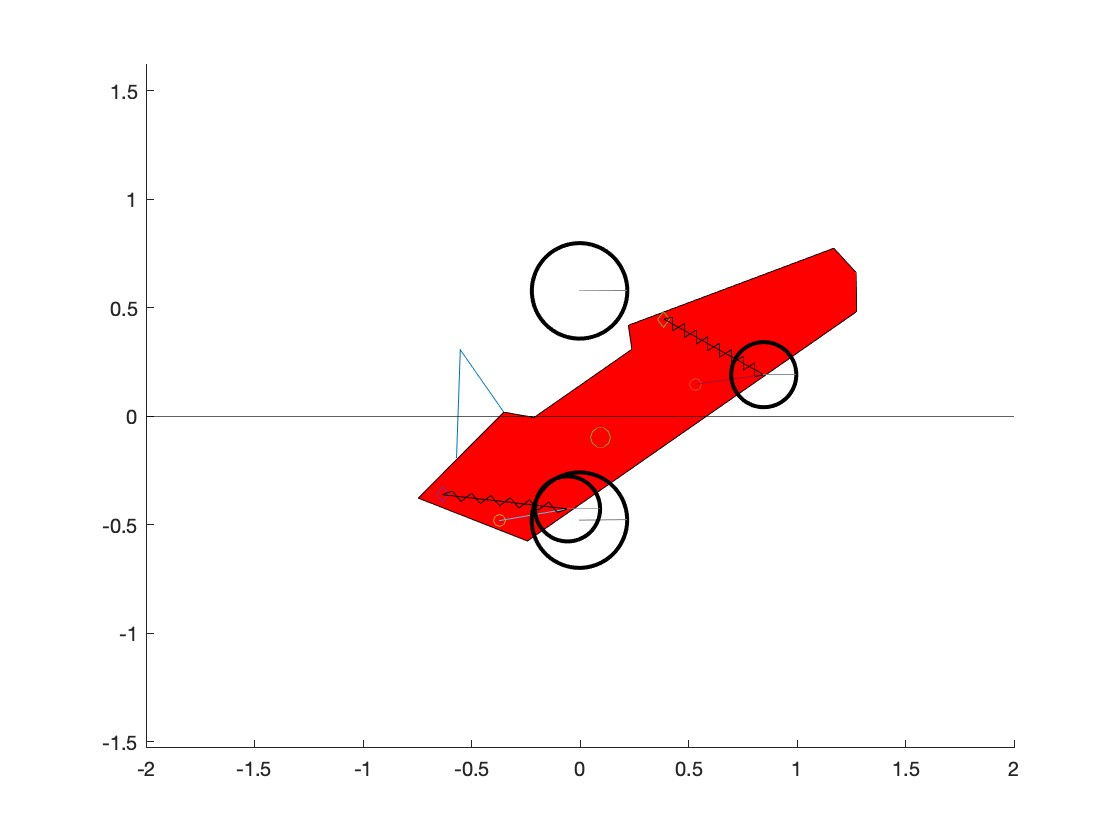
\includegraphics[scale=0.235]{images/mode1.jpg}
    \caption{Eigenmode Configuration 1}
    %label always in the end
    \label{fig:mode_1}
\end{figure}

\begin{figure}[ht]
    \centering
    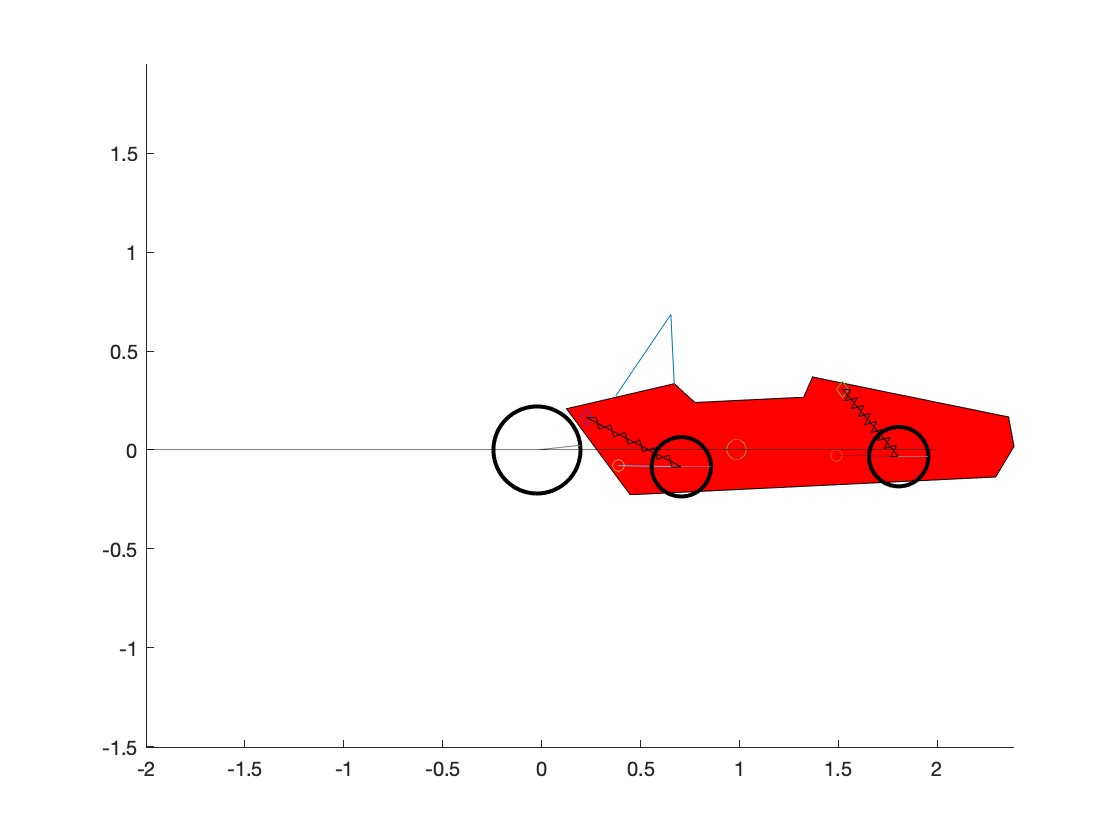
\includegraphics[scale=0.235]{images/mode2.jpg}
    \caption{Eigenmode Configuration 2}
    %label always in the end
    \label{fig:mode_2}
\end{figure}

\begin{figure}[ht]
    \centering
    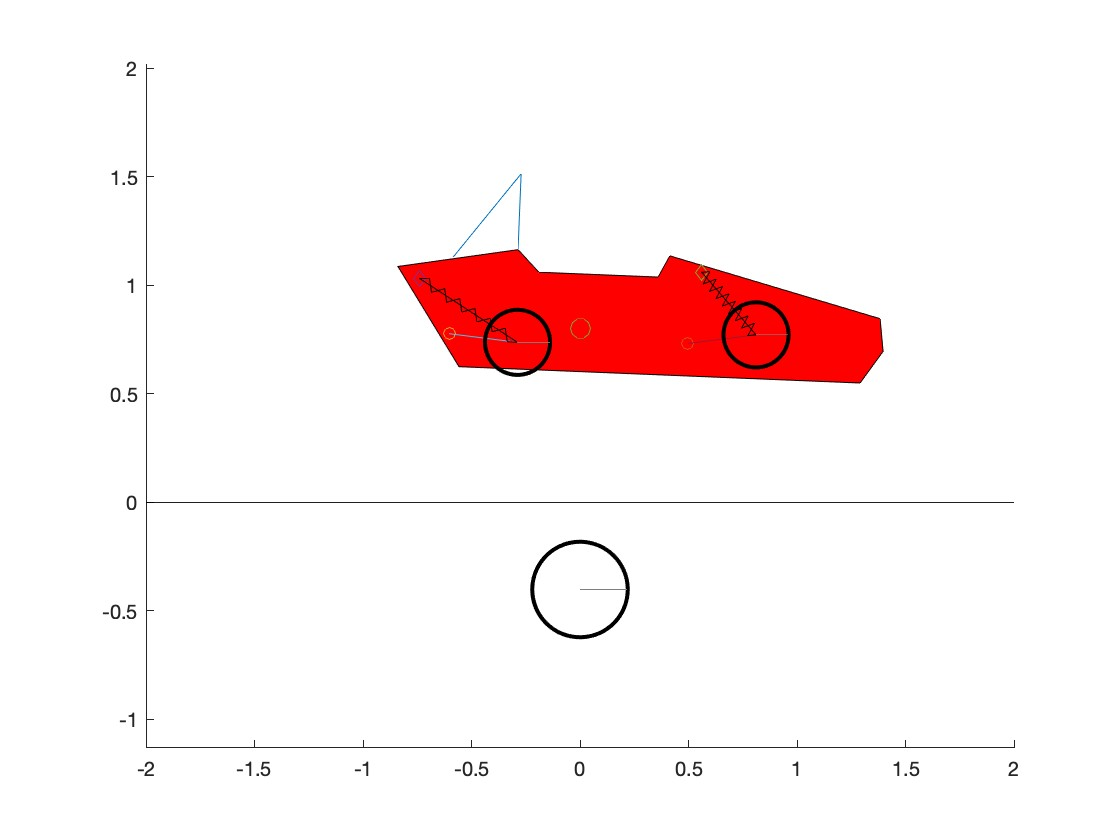
\includegraphics[scale=0.235]{images/mode3.jpg}
    \caption{Eigenmode Configuration 3}
    %label always in the end
    \label{fig:mode_3}
\end{figure}

If only these could be explained.

\subsubsection{DONE}
\subsubsection{Mode Shapes}

\subsection{Drag and Damping}
\subsubsection{Damping}
The contributions to the damping force are:
\begin{equation}
    \begin{split}
        Q_{\text{suspension back}} = \begin{pmatrix}
            Q_{\text{susb(1)}}\\
            0\\
            0\\
            0\\
            0\\
            0\\
            0\\
            0\\
            0\\
            Q_{\text{susb(2)}}\\
            0
        \end{pmatrix}
    \end{split}
\end{equation}
Which has a contribution towards the rotation of the frame and the rotation of the back link. Both of these contributions have a negative sign which makes sense as the suspension of the back tire will lift the back wheel resulting in a rotation of the bar and the frame in negative Z direction.

Analogous for the front suspension:
\begin{equation}
    \begin{split}
        Q_{\text{suspension front}} = \begin{pmatrix}
            Q_{\text{susf(1)}}\\
            0\\
            0\\
            0\\
            0\\
            0\\
            0\\
            0\\
            0\\
            0\\
            Q_{\text{susf(2)}}
        \end{pmatrix}
    \end{split}
\end{equation}
Therefore the front suspension force leads to an impact on the frame angle and the front link angle.

Note: these two suspension forces come from the spring approximation of the reality.

\begin{equation}
    \begin{split}
        Q_\text{tire back} = \begin{pmatrix}
            0\\
            0\\
            0\\
            0\\
            0\\
            0\\
            0\\
            Q_\text{tB(9)}\\
            0\\
            0\\
            0
        \end{pmatrix}
    \end{split}
\end{equation}
The back tire contact force has an impact on the elevation of the back tire.

\begin{equation}
    \begin{split}
        Q_\text{tire front} = \begin{pmatrix}
            0\\
            0\\
            0\\
            0\\
            0\\
            0\\
            0\\
            Q_\text{tF(9)}\\
            0\\
            0\\
            0
        \end{pmatrix}
    \end{split}
\end{equation}
This has an impact on the elevation of the front tire component.
\subsubsection{Drag Forces}
\begin{equation}
    \begin{split}
        Q_\text{drag} =
        \begin{pmatrix}
            0\\
-(63*\dot x_\text{fr}^2)/100\\
                0\\
                0\\
                0\\
                0\\
                0\\
                0\\
                0\\
                0\\
                0
        \end{pmatrix}
    \end{split}
\end{equation}
This is the aerodynamic drag on the system. This can be nicely seen as there is only a negative component in the second row (depending on the velocity in this direction scquared) which corresponds to the x movement of the frame. Thus we have aerodynamic drag in that direction.

\begin{equation}Q_\text{friction wheels} = 
    \begin{pmatrix}
        0\\
        0\\
        0\\
-\dot\theta_\text{wF}^3/50000\\
-\dot\theta_\text{wB}^3/50000\\
        0\\
        0\\
        0\\
        0\\
        0\\
        0
    \end{pmatrix}
\end{equation}
Here we can nicely see friciton drag impacting the rotation of the front and the back wheel.

Lastly we have for the torque:
\begin{equation}
    Q_\text{wheel} = 
    \begin{pmatrix}
        0\\
        0\\
        0\\
        0\\
        -300\\
        0\\
        0\\
        0\\
        0\\
        0\\
        0
    \end{pmatrix}
\end{equation}
Representing the load applied in negative Z direction on the back wheel to make the car drive to the right.

\subsection{Nonlinear Time Integration}
\subsubsection{}
\subsubsection{}
\subsubsection{}
\subsubsection{}
\subsection{Adding Wings}
\subsubsection{}
\subsubsection{}
\subsubsection{}
\subsubsection{}
\subsection{Harmonic Response}


